% !TEX root = thesis-ex.tex
% a phase of matter that provides access to the otherwise confined partons.
%This is the state of matter as it existed in the early universe and having a thermodynamic description of the QGP can provide insight into its transition to hadronic matter, and help explain the QCD phase diagram shown in Figure~\ref{}.

Heavy ion collisions are a tool that can be used as a tool to study the quark-gluon plasma (QGP) \cite{SHURYAK198071}.
In a heavy ion collision, the colliding nuclei are accelerated to relativistic energies and due to relativistic length contraction, form discs.
In the case of a \pbpb\ collision, the relativistic $\gamma$ factor is approximately 3000. 
Each nucleus contains many colored quarks and antiquarks, with three more quarks than anti-quarks per nucleon, with the $q\bar{q}$ popping in and out of the vacuum due to quantum fluctuations.
These $q\bar{q}$ pairs are sources of transverse color fields and the corresponding force carriers, the gluons.

%move to jets?
%The probability distributions of these partons within a proton are given by the parton distribution functions (PDFs) \cite{Placakyte:2011az}. 
%These PDFs given as $f(x, Q^2)$ and shown in Figure~\ref{fig:pdfs} are functions of the longitudinal momentum fraction $x$ and the scale of the hard interaction, $Q$. 
%They are determined via fits to data from Deep Inelastic Scattering experiments and form the cornerstone of any theoretical prediction for hadron colliders.
%
%\begin{figure}[htbp]
%\begin{center}
%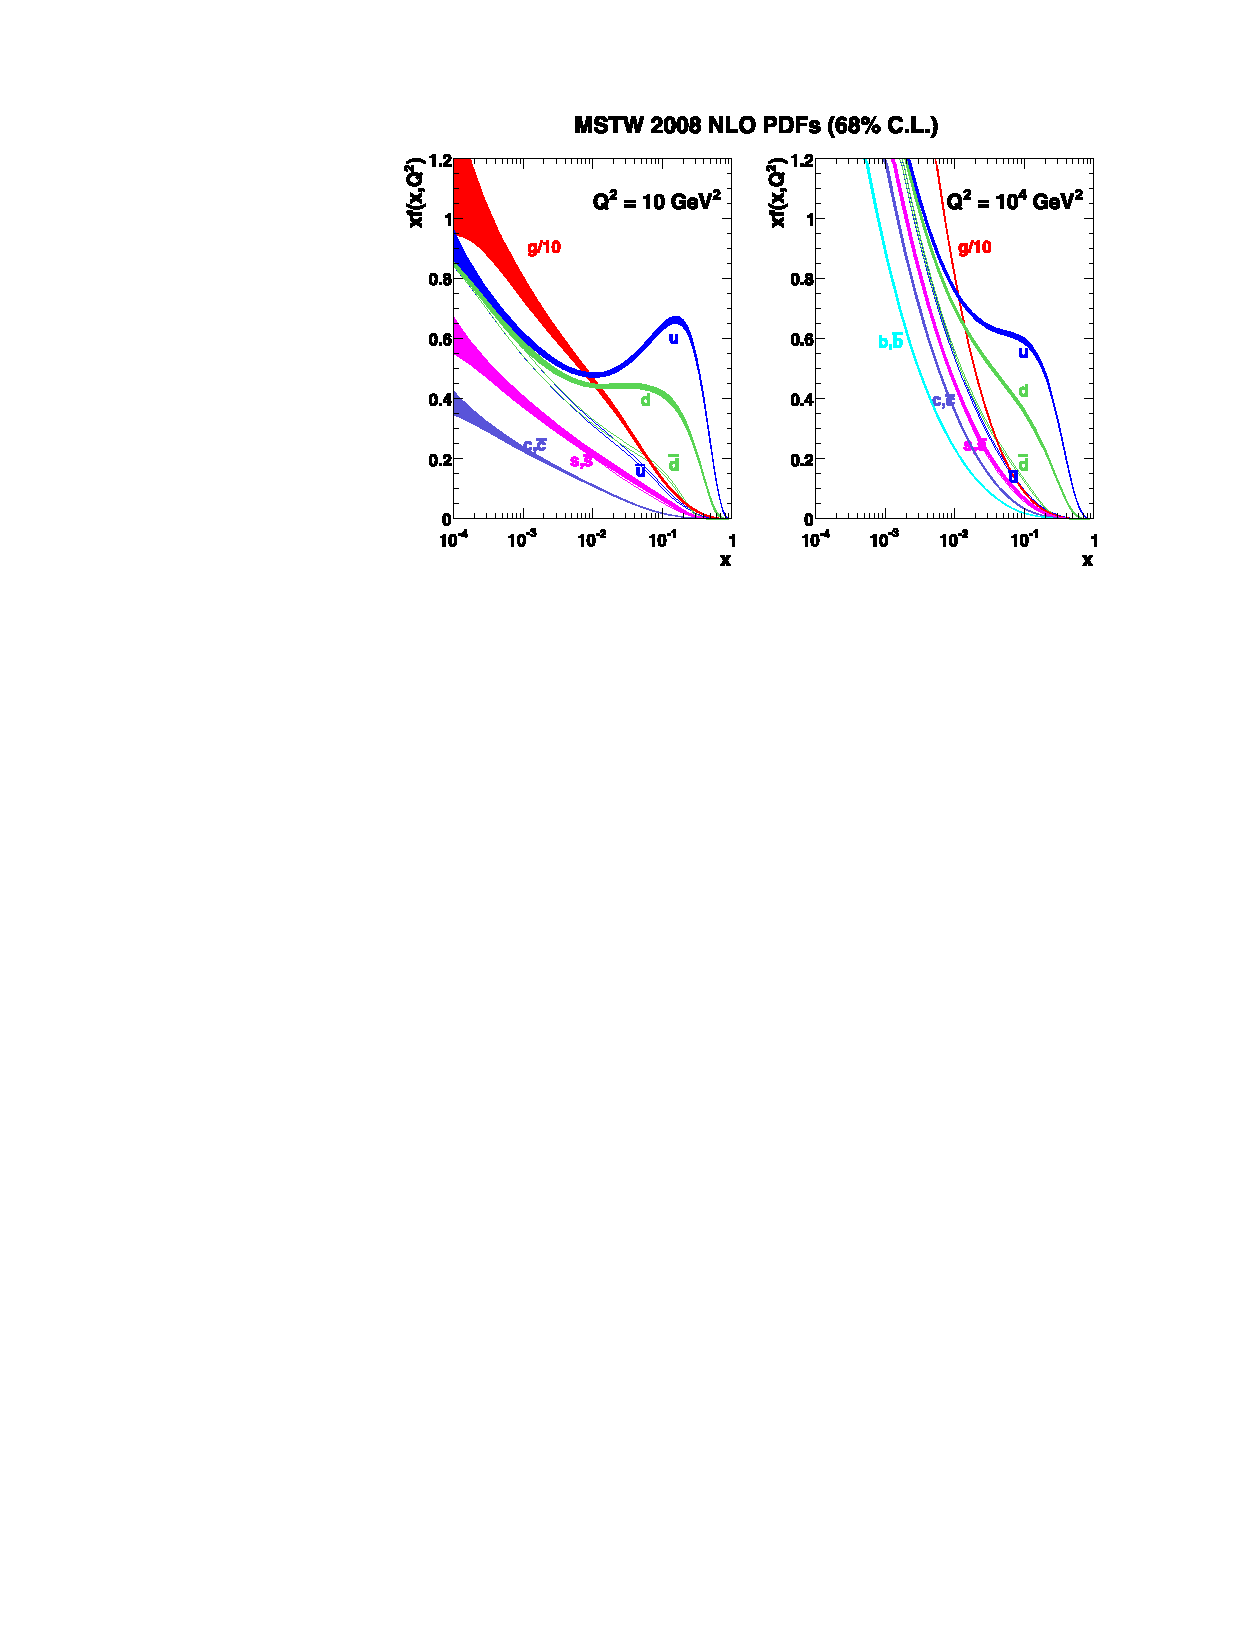
\includegraphics[width=0.65\textwidth]{figures/theory/pdfs}
%\caption{The MSTW (Martin-Stirling-Thorne-Watt) 2008 PDFs at next to leading order NLO, at two scales: $Q^2 = 10 \rm{GeV}^2$ and $Q^2 = 10^4 \rm{GeV}^2$.
%Figure from Reference \cite{Martin2009}.}
%\label{fig:pdfs}
%\end{center}
%\end{figure}

When these pancake-like discs collide, their color fields interact and there is a color charge exchange, producing longitudinal color fields that fill the space between the receding discs.
%The energy density of the collision region is given by the Bjorken energy density of the QGP can be derived using \cite{PhysRevD.27.140}:
%
%\begin{align}
%\varepsilon = \frac{1}{A_{\rm{T}} t} \frac{d \Et}{dy}
%\end{align}
%where $A_\rm{T}$ represents the transverse overlap area and $d\Et/dy$ is the transverse energy per unit rapidity (see Section~\ref{sec:quantities} for a definition of rapidity). 
%where $d\Nch/d\eta$ is the number of charged particles produced per unity pseudorapidity, $d\Et/d\eta$ is the transverse energy per unit pseudorapidity, $\tau_0$ is the thermalization time, $R$ is the nuclear radius, and $\Et/N \approx 1$ GeV is the transverse energy per emitted particle.
%As shown in Figure~\ref{fig:energyDensity}, the energy density at the LHC was measured to be approximately 15 $\mathrm{GeV} / \mathrm{fm}^3$, much higher than the values measured at RHIC \cite{Adcox:2004mh, Krajcz_r_2011}.
%
%
%\begin{figure}[htbp]
%\begin{center}
%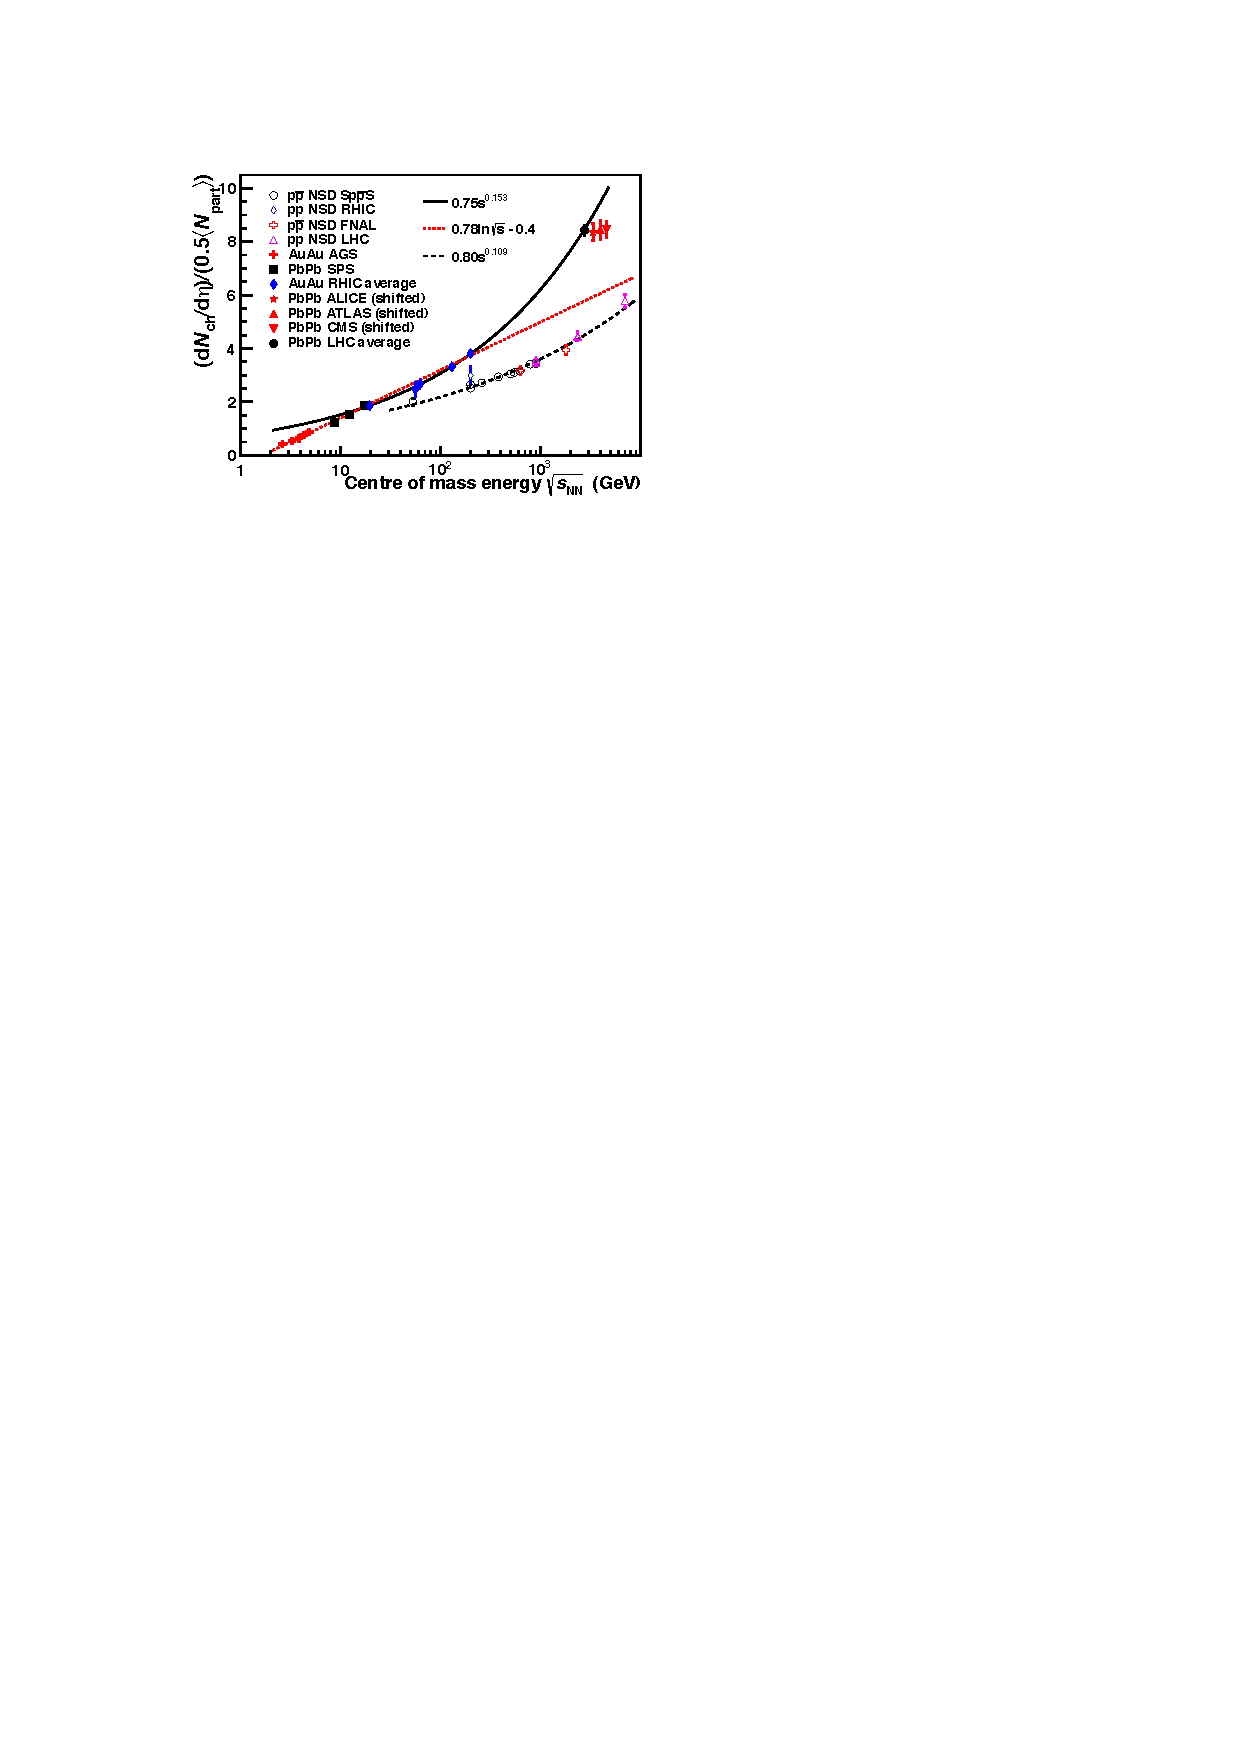
\includegraphics[width=0.65\textwidth]{figures/theory/energyDensity}
%\caption{$d\Nch/d\eta$ per colliding nucleon pair as a function of collision energy in \pp\ and nucleus-nucleus collisions \cite{Muller:2012zq}.}
%\label{fig:energyDensity}
%\end{center}
%\end{figure}
%
%
The energy densities attained at RHIC and the LHC are as low as $1 \rm{GeV}/\rm{fm}^3$ \cite{PhysRevC.93.024901} and $12 \rm{GeV}/\rm{fm}^3$ \cite{PhysRevC.94.034903, PhysRevLett.109.152303} respectively, both of which are above the $0.2 - 1 \rm{GeV}/\rm{fm}^3$ energy density range required to form the QGP \cite{Karsch2002, PhysRevD.90.094503}.

%Lattice QCD calculations in thermodynamics show that at these energies, the partons produced in the collision cannot be treated as a collection of distinct hadrons.

%In fact, these partons are strongly coupled to each other and form a medium called the Quark Gluon Plasma (QGP) \cite{???}.
%In a heavy ion collision, the experimenter can only tune the size of the colliding nuclei, and the energy that they are being collided at.
%There is no experimental control over the impact parameter or the structure functions that dictate the momentum distribution of nucleons within the nucleus.
%These have to be determined event by
% most of the partons are participate in soft interactions that do not involve large transverse momentum transfer, and are hence scattered only at small angles.
%A small fraction of the colliding partons however do undergo hard perturbative interactions and lead to particles with large transverse momenta.
%These subsequently decaying to $q\bar{q}$ pairs.
%The QGP can be described by relativistic hydrodynamics, and has a viscosity to entropy ratio that is almost at the theoretical minimum of of $\eta / S = 1/4\pi$ \cite{5,6, check126}.


After the collision the energy density between the receding nuclei starts to decrease as the QGP cools and expands.
This process, seen in Figure~\ref{fig:qgp_form}, continues till the energy density drops to below that within a hadron and the fluid ``hadronizes''.
These individual hadrons briefly scatter off of each other before they freely fly towards the detector (freeze-out).

%Once formed, the QGP flows hydrodynamically, with the initial pressure driving the expansion and the subsequent cooling.
% It is to be noted that there is QGP continuously formed in the wake of the nuclei since the partons produced at large rapidities are highly relativistic and 

\begin{figure}[htbp]
\begin{center}
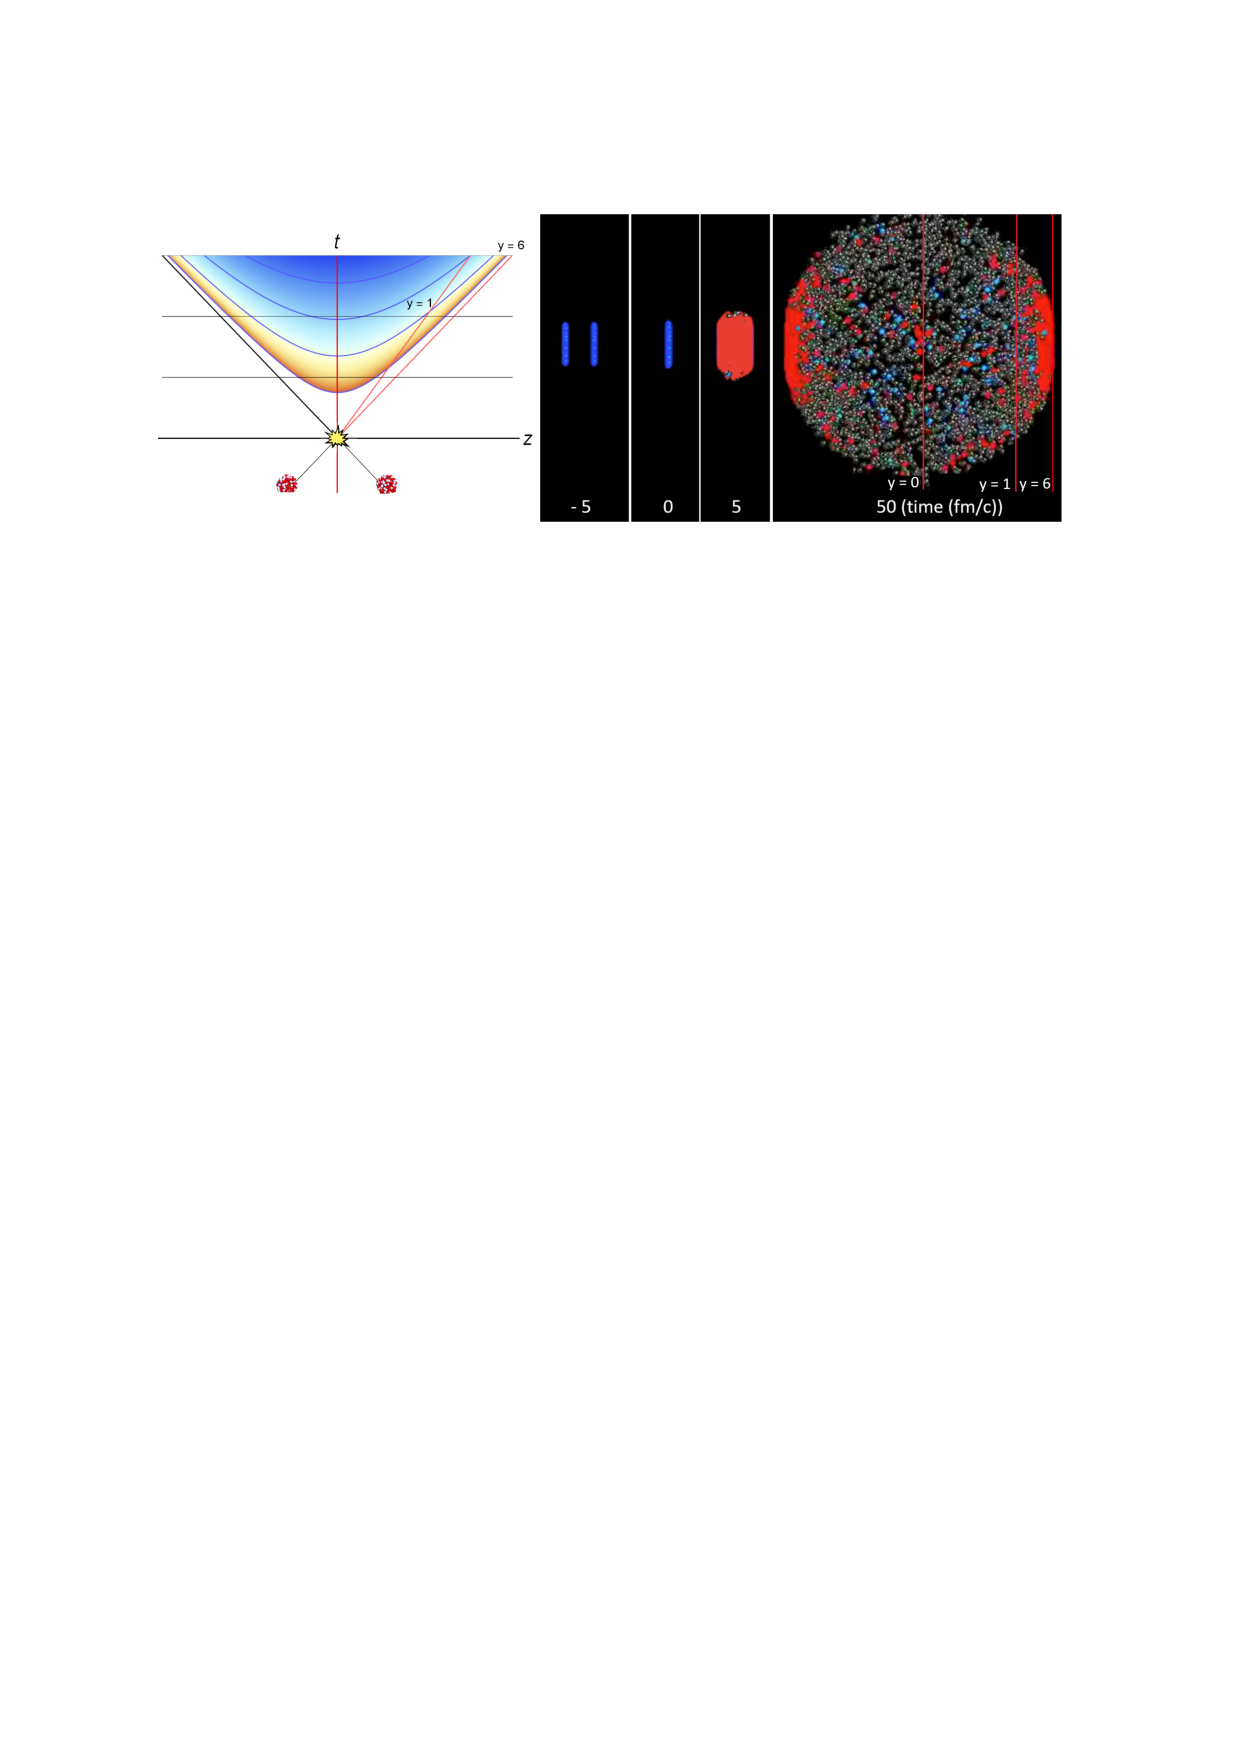
\includegraphics[width=0.85\textwidth]{figures/theory/qgp_formation}
\caption{(left) Space-time diagram for a heavy ion collision.
The color is indicative of the temperature of the QGP formed.
(right) Snapshots of a heavy ion collision at $\sqrtsnn = 2.76$ TeV at different times.
The Lorentz contracted nuclei are in blue while the QGP is in red.
Figure from Reference \cite{Busza:2018rrf}.}
\label{fig:qgp_form}
\end{center}
\end{figure}

While Figure~\ref{fig:qgp_form} shows snapshots of a head on (central) collision between two large nuclei, it is possible to have collisions where the impact parameter is larger and hence the overlap region is smaller.
These collisions, called peripheral collisions, qualitatively undergo the same process described above, with the size and shape of the QGP being different.
A schematic of both central and peripheral collisions is shown in Figure~\ref{fig:collision_centrality}.

\begin{figure}[htbp]
\begin{center}
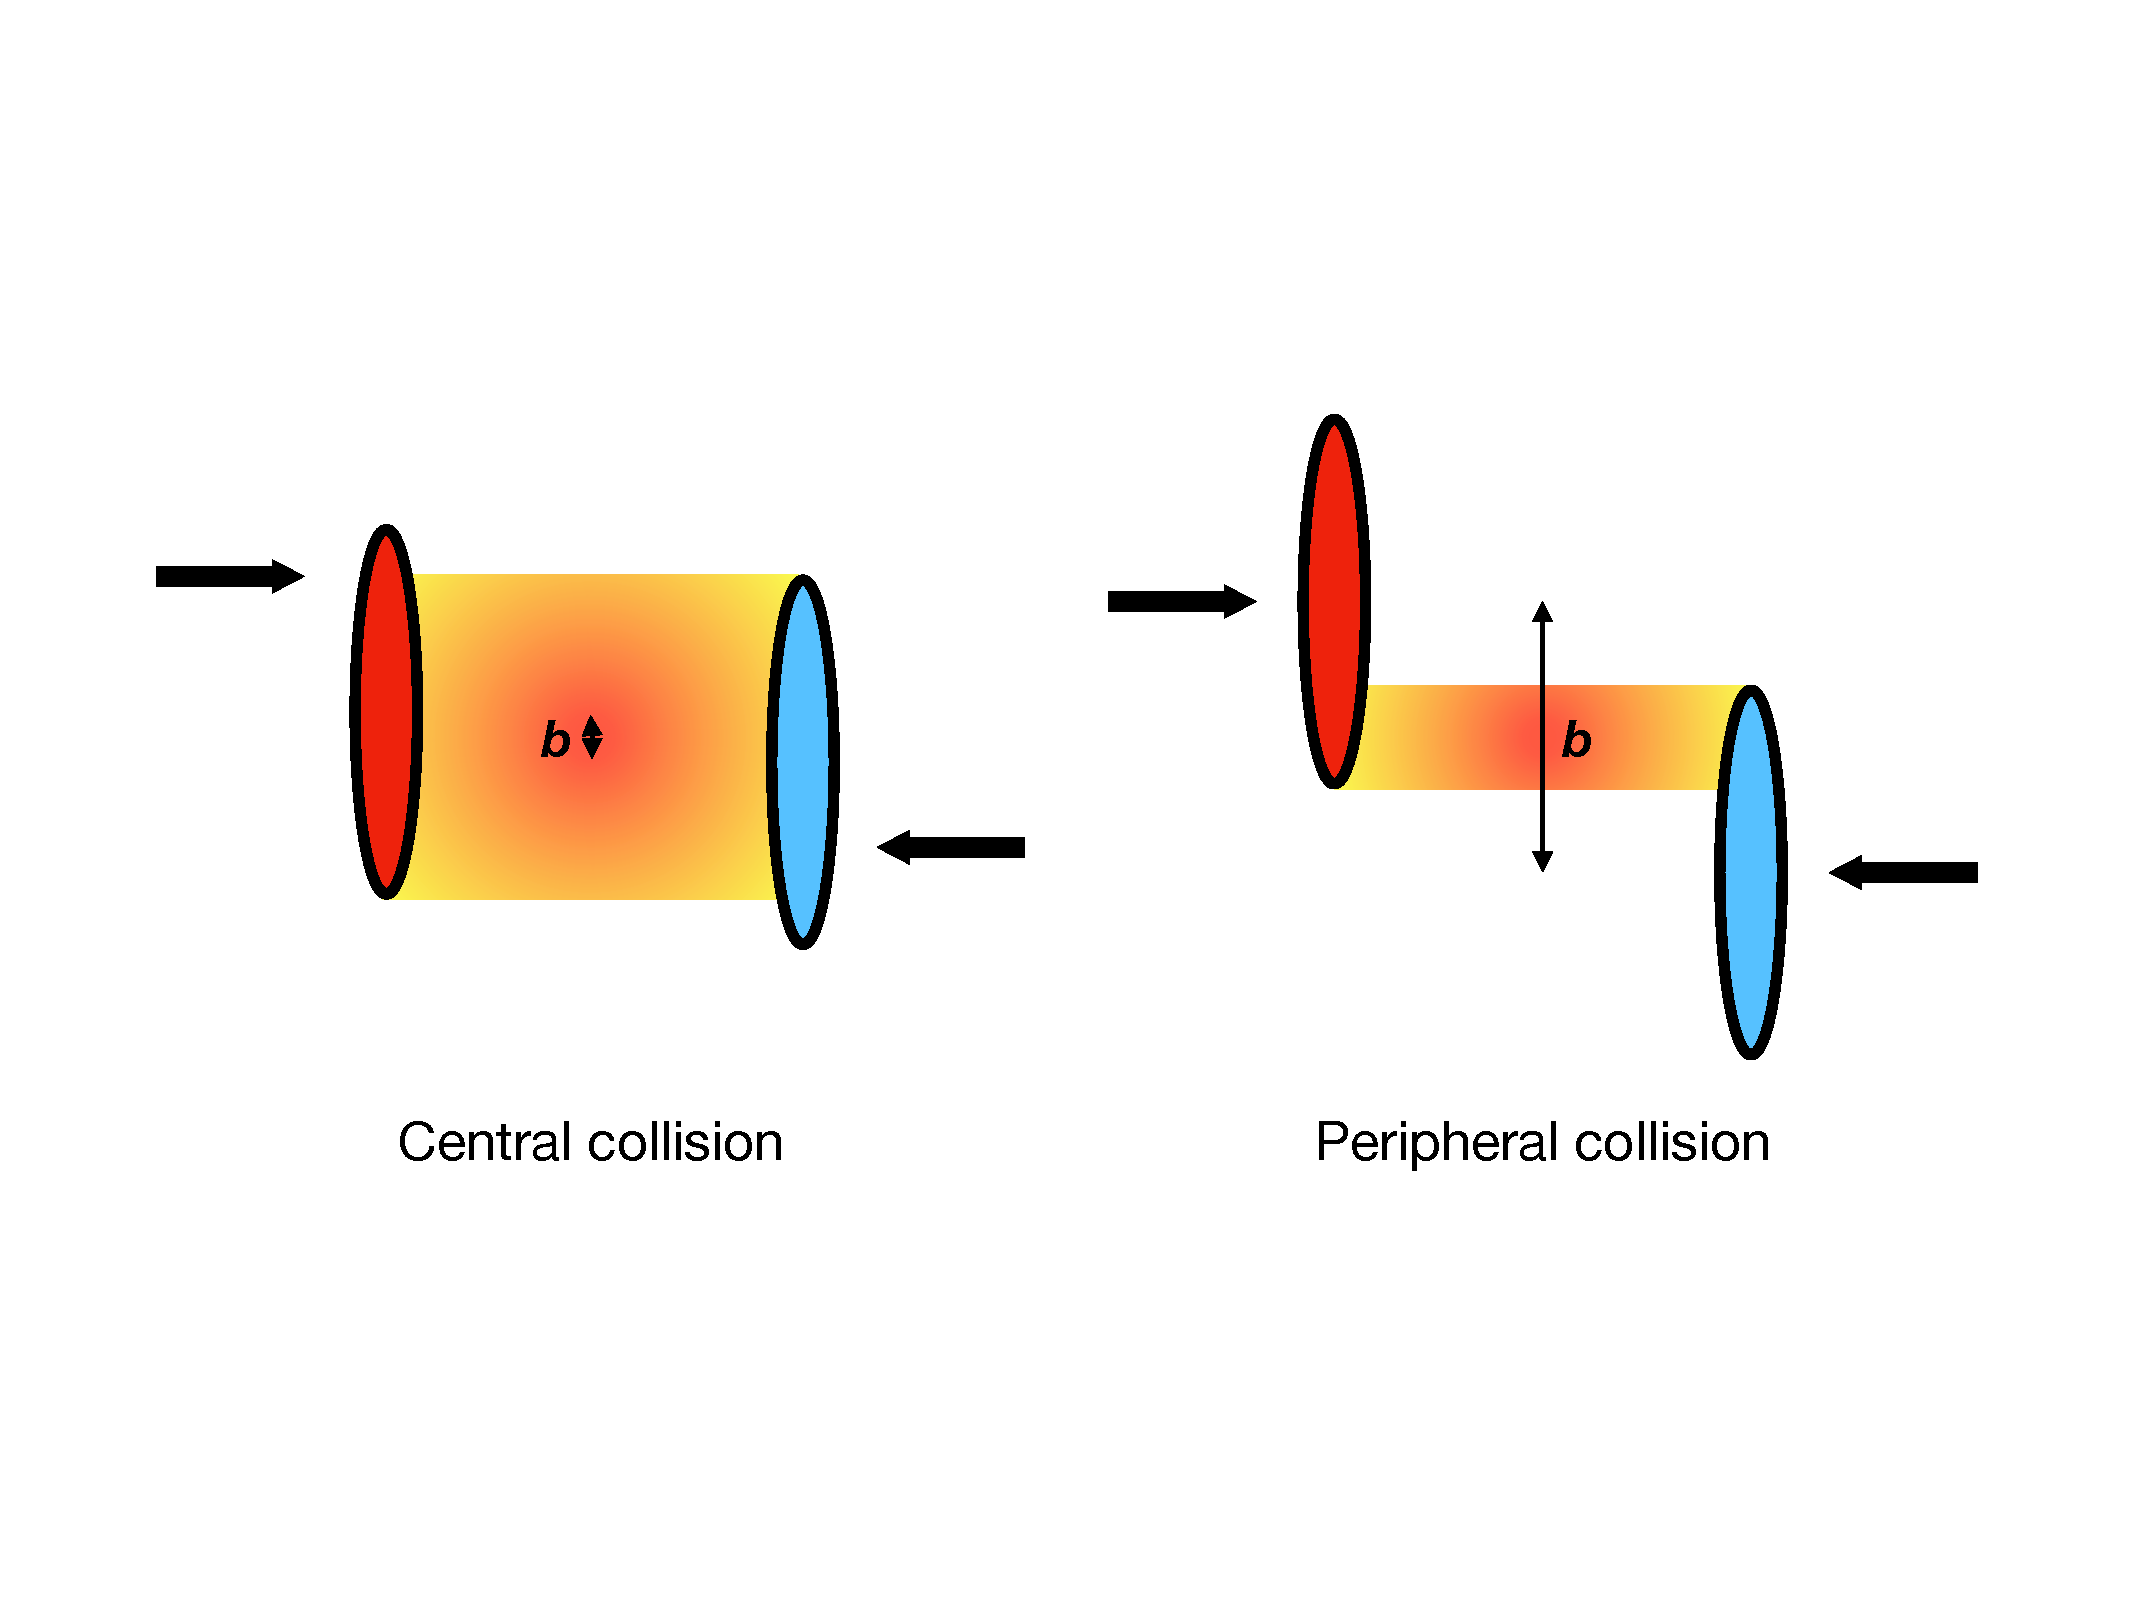
\includegraphics[width=0.85\textwidth]{figures/theory/collision_centrality}
\caption{A schematic of central (left) and peripheral (right) heavy ion collisions.
The impact parameter is given by $b$.}
\label{fig:collision_centrality}
\end{center}
\end{figure}

% In fact, peripheral collisions are very similar to proton-proton collisions, with differences coming mainly from nuclear PDFs.

The basic parameters of a heavy ion collision such as the number of participants \Npart\ and number of binary collisions \Ncoll\ can be determined using the Glauber Monte Carlo simulations \cite{glauberArticle, glauberMisc}.
This technique considers a nucleus-nucleus collision as a collection of independent binary nucleon-nucleon collisions; the colliding nuclei are modeled as a set of uncorrelated nucleons being positioned within the nucleus based on a the nuclear density function uniform in azimuthal and in polar angles.
The nuclear density function in this model is a parameterized Fermi distribution given by: 

\begin{align}
\rho(r) = \rho_0 \frac{1 + w (r/R)^2}{1+e^{\frac{r-R}{a}}}
\end{align}
where $\rho_0$ is the nucleon density, $R$ is the nuclear radius, $a$ is the skin depth, $w$ corresponds to deviations from a circular shape and is typically zero for larger nuclei like Cu, W, Au, Pb, and U.
For the Pb nuclei used at the LHC, $w = 0$, $R = 6.62$ fm and $a =0.55$ fm \cite{DEVRIES1987495}.
The nuclear density distribution for Au and Cu is shown in Figure~\ref{fig:nuclearDensity}.

\begin{figure}[htbp]
\begin{center}
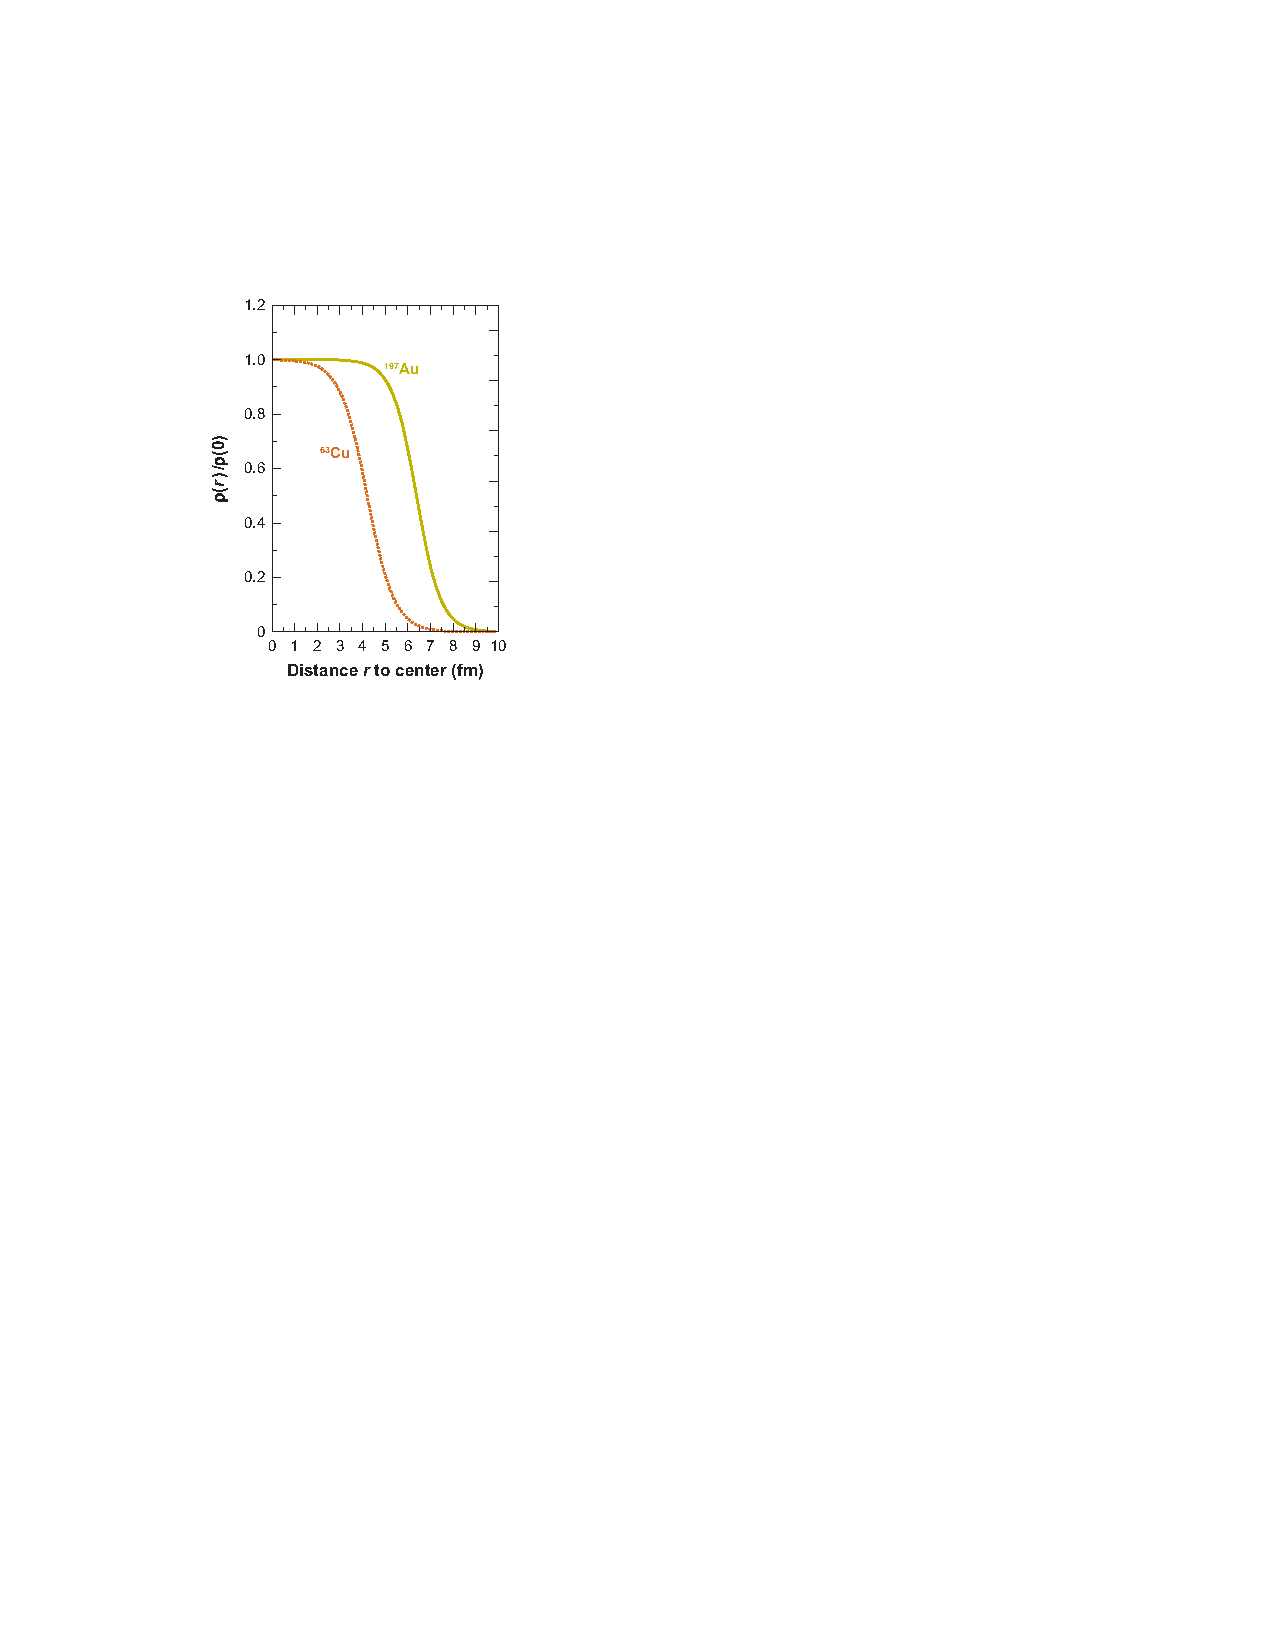
\includegraphics[width=0.35\textwidth]{figures/theory/nuclearDensity}
\caption{ The nuclear density distributions for nuclei used at RHIC: Cu ($w = 0$, $R = 4.2$ fm and $a =0.48$ fm)  and Au ($w = 0$, $R = 6.38$ fm and $a =0.535$ fm) \cite{DEVRIES1987495}.
Figure taken from Ref.~\cite{doi:10.1146/annurev.nucl.57.090506.123020}.}
\label{fig:nuclearDensity}
\end{center}
\end{figure}

They are then arranged with a random impact parameter $b$ based on the distribution $d\sigma/d b = 2\pi b$ and projected onto the $x-y$ plane as shown in Figure~\ref{fig:glauberMC}.
They are then made to travel on straight trajectories, colliding if $d \leq \sqrt{\sigma_{\mathrm{inel}}^{\mathrm{NN}}/ \pi}$, where $d$ is the distance between the nucleons in a plane transverse to the beam axis and $\sigma_{\mathrm{inel}}^{\mathrm{NN}}$ is the inelastic scattering cross section. \cite{doi:10.1146/annurev.nucl.57.090506.123020, Alver:2008aq}

\begin{figure}[htbp]
\begin{center}
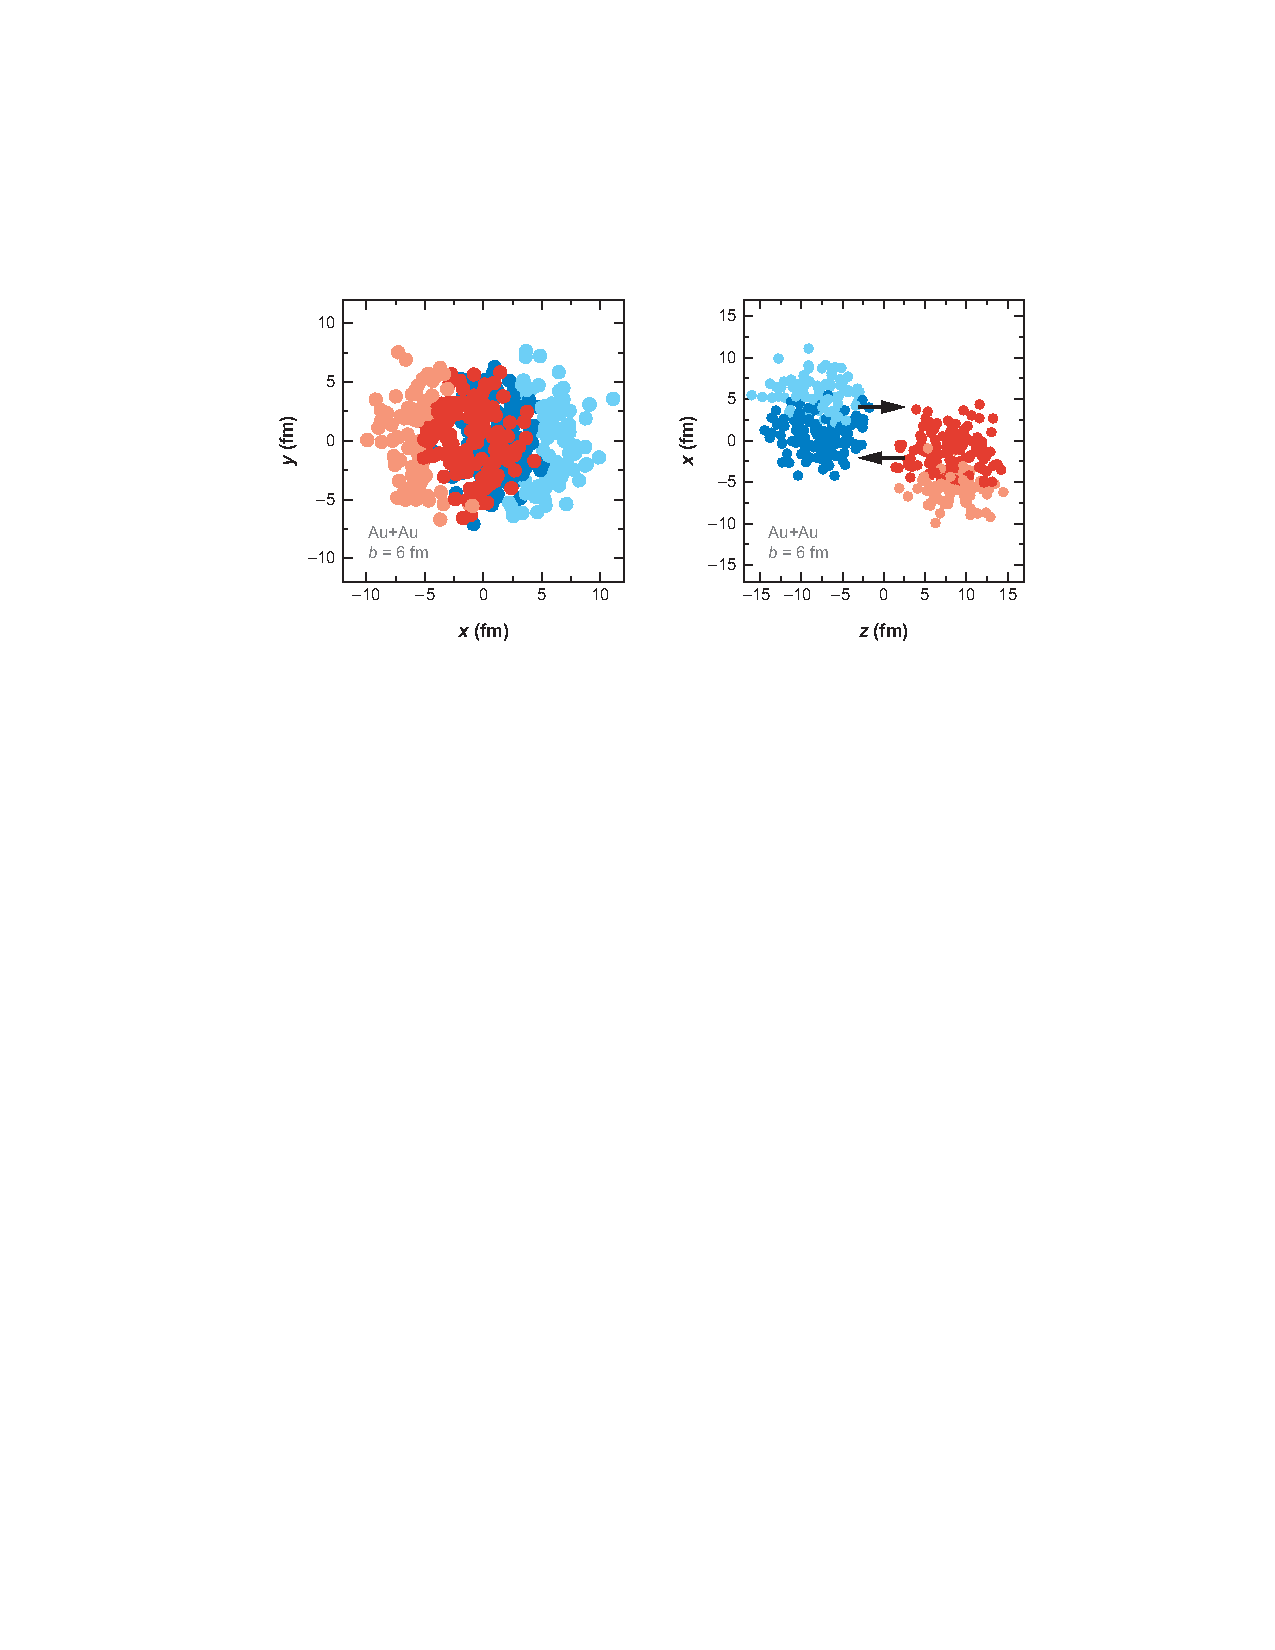
\includegraphics[width=0.85\textwidth]{figures/theory/glauberMC}
\caption{A Glauber Monte Carlo event for $Au+Au$ at \sqrtsnn = 200 geV with impact parameter of 6 fm viewed in the (left) transverse plane and (right) along the beam axis.
Darker circles represent the participating nucleons.
Taken from \cite{doi:10.1146/annurev.nucl.57.090506.123020}.}
\label{fig:glauberMC}
\end{center}
\end{figure}



An important parameter for colliding nuclei A and B with $A$ and $B$ nucleons is the thickness function $T_{AB}$.
It describes the effective overlap area in which specific nucleons in the two colliding nuclei can interact.
It can be defined in terms of the probability per unit area of a given nucleon being located at a particular distance $s$ within the nucleus.
For the colliding nuclei $A$ and $B$, this is given by $T_{A}({\bf{s}}) = \int \rho_A ({\bf{s}}, z_A) dz_{A}$ and $T_{B}({\bf{s}}) = \int \rho_B ({\bf{s}}, z_B) dz_{B}$.
Then, $T_{AB}$ is given by

\begin{align}
T_{AB}({\bf b}) = \int T_{A} ({\bf s}) T_{B} ({\bf s-\bf b}) d^2 s
\end{align}
The probability of then having $n$ interactions between nuclei $A$ and $B$ is given by the binomial distribution:

\begin{align}
P(n, { \bf b}) = {{AB} \choose {n}} \Big[T_{AB}( {\bf b} ) \sigma_{\mathrm{inel}}^{\mathrm{NN}} \Big]^n \Big[ 1 - T_{AB}( {\bf b} ) \sigma_{\mathrm{inel}}^{\mathrm{NN}} \Big]^{AB-n}
\end{align}
where the first term is the number of combinations for finding $n$ collisions from $AB$ possibilities, the second term is the probability for having exactly $n$ collisions, and the last term the probability of $AB-n$ misses.
Then the total probability of an interaction between A and B is:

\begin{align}
\frac{d^2  \sigma_{\mathrm{inel}}^{\mathrm{AB}} }{db^2} \equiv p_{\mathrm{inel}}^{\mathrm{AB}} (b) = \sum_{n=1}^{AB} P(n, {\bf b}) = 1- \Big[ 1 - T_{AB}( {\bf b} ) \sigma_{\mathrm{inel}}^{\mathrm{NN}} \Big]^{AB}
\end{align}

Then the total cross section is given by

\begin{align}
\sigma_{\mathrm{inel}}^{\mathrm{AB}} = \int_0^\infty 2\pi b db \Bigg[ 1- \Big( 1 - T_{AB}( {\bf b} ) \sigma_{\mathrm{inel}}^{\mathrm{NN}}  \Big)^{AB} \Bigg]
\end{align}
and \Ncoll\ and \Npart are given by \cite{Kharzeev:2000ph, Bialas:1976ed}:

\begin{align}
\Ncoll (b) = & \sum_{n=1}^{AB} n P(n, b) =  AB \times T_{AB}(b) \sigmainel \\
\Npart (b) = & A \int T_A ({\bf s}) \Big[ 1 - \big(1-T_B ({\bf s - b}) \sigmainel \big)^B \Big] d^2 s \\
+ & B \int T_B ({\bf s-b}) \Big[ 1 - \big(1-T_A ({\bf s}) \sigmainel \big)^A \Big] d^2 s \nonumber
\end{align}
The correlation between \Ncoll\ and \Npart\ can be seen in Figure~\ref{fig:NcollNpart}:

\begin{figure}[htbp]
\begin{center}
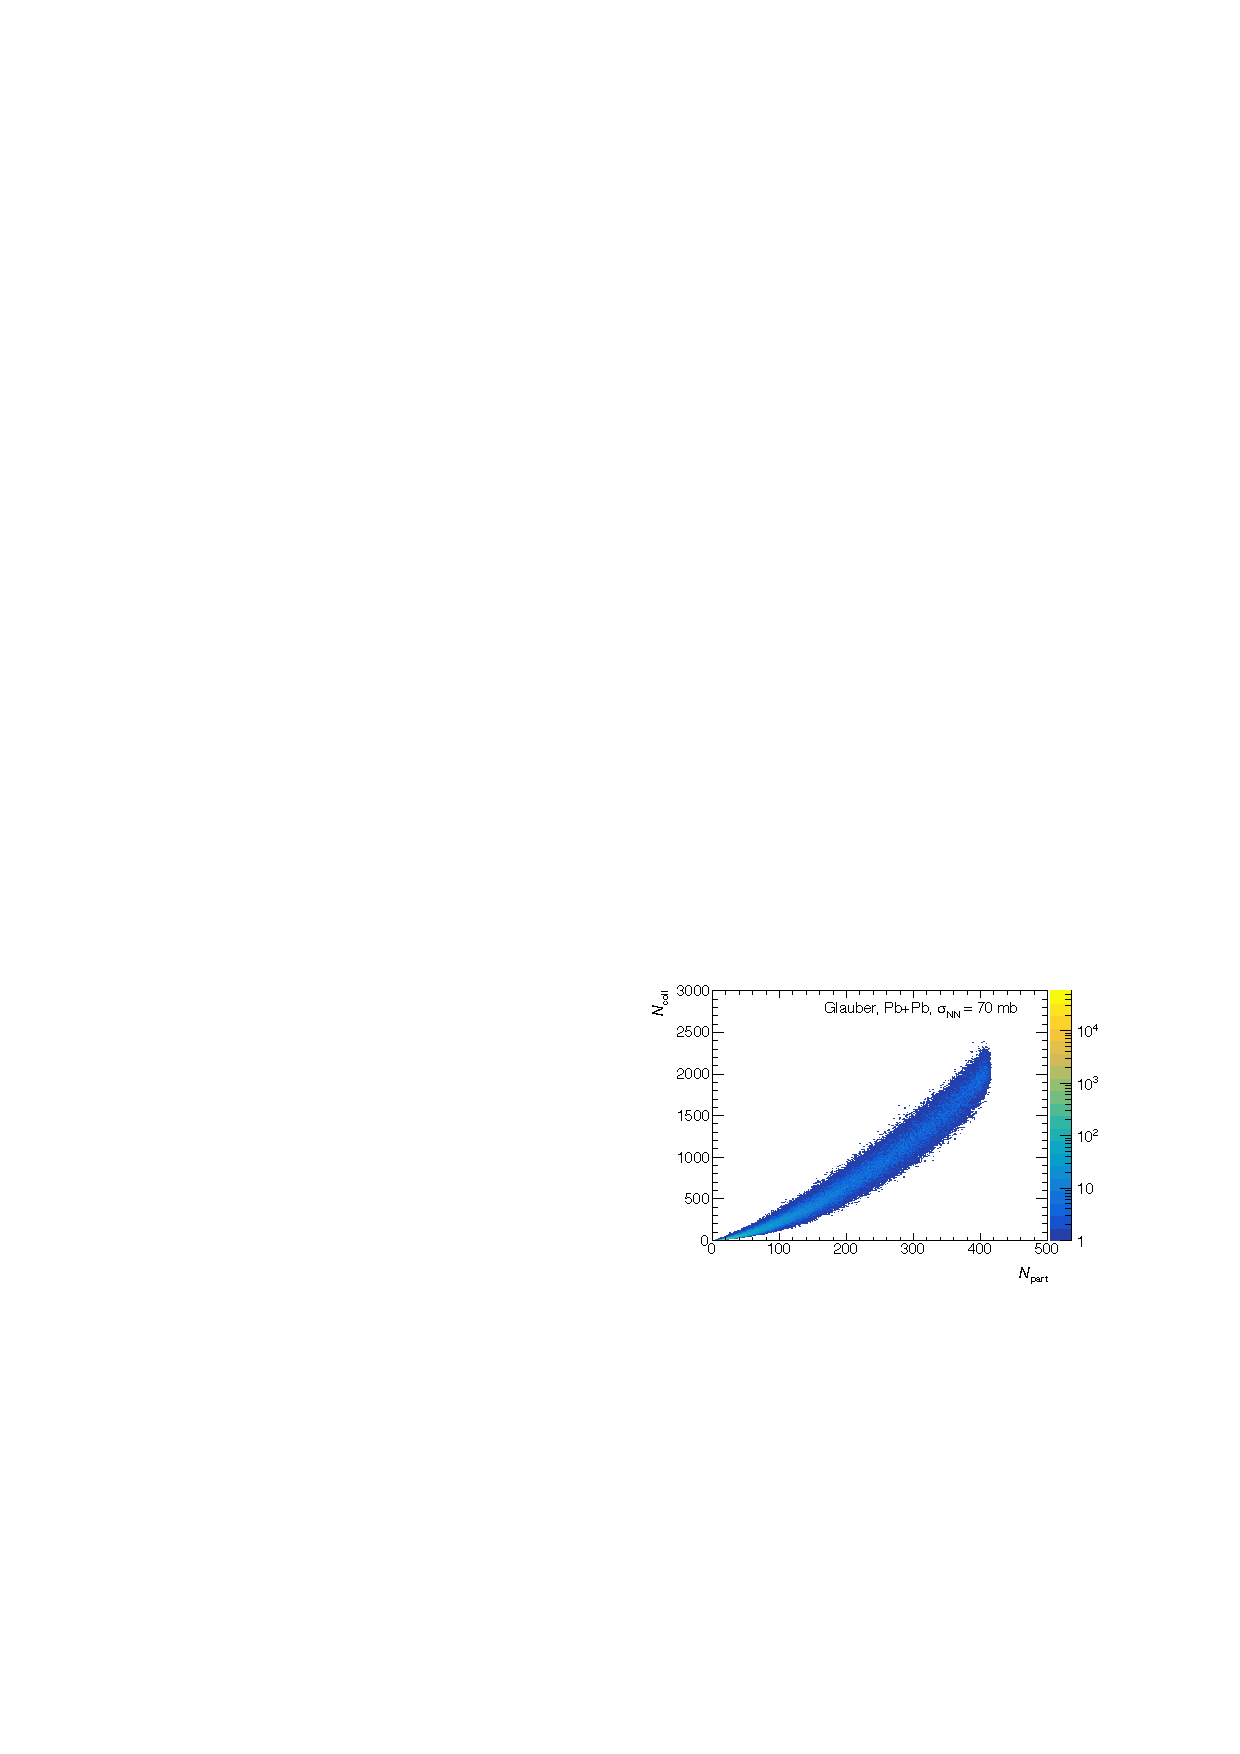
\includegraphics[width=0.55\textwidth]{figures/theory/NcollNpart}
\caption{The $\Ncoll-\Npart$ correlation for \pbpb\ collisions at \sqrtsnn\ = 5.02 TeV.
Taken from \cite{Perepelitsa:2212936}.}
\label{fig:NcollNpart}
\end{center}
\end{figure}

The charged particle multiplicity $N_{\mathrm{ch}}$ along with the combination of \Npart\ and impact parameter $b$ can be used to determine the centrality of a heavy ion event.
An example of this is shown in Figure~\ref{fig:cent_estimate}.

\begin{figure}[htbp]
\begin{center}
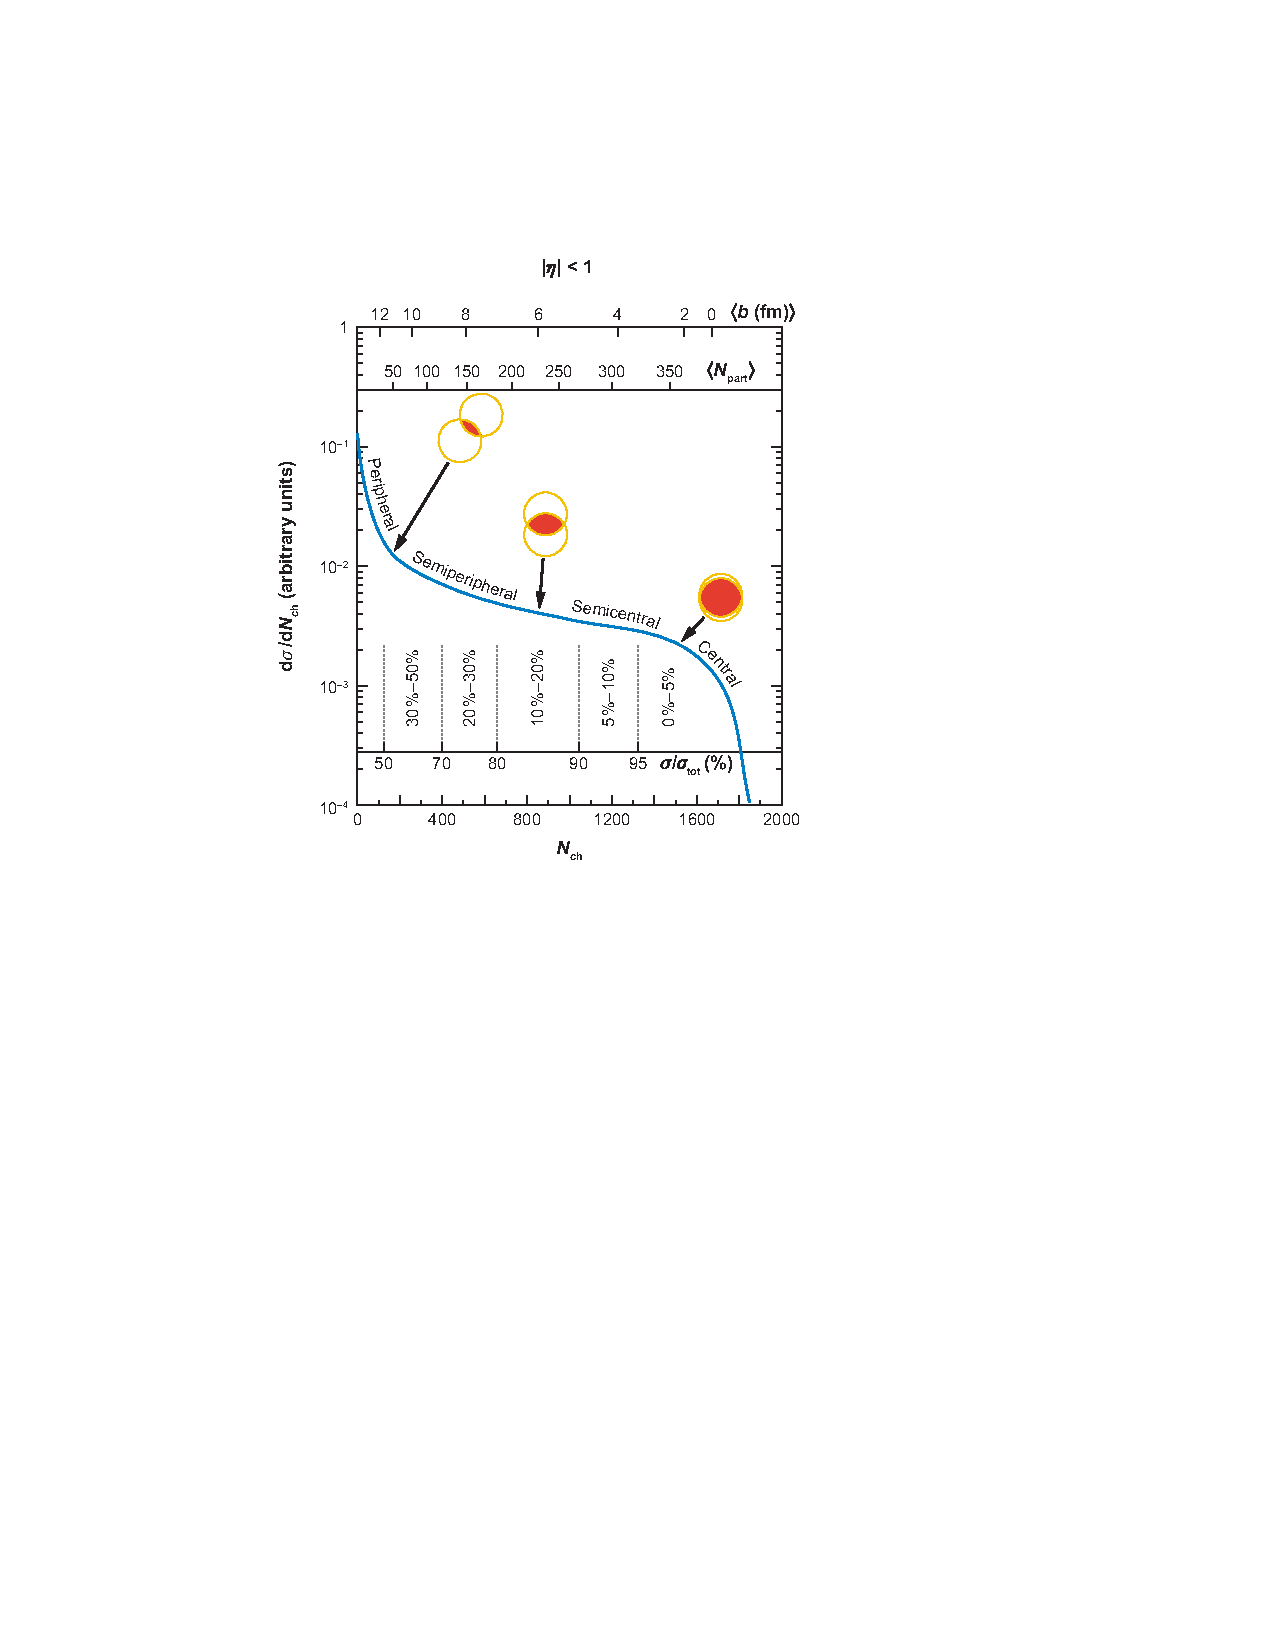
\includegraphics[width=0.45\textwidth]{figures/theory/cent_estimate}
\caption{The correlation between the observable \Nch\ and \Npart\ to determine the centrality distribution.
Taken from \cite{doi:10.1146/annurev.nucl.57.090506.123020}.}
\label{fig:cent_estimate}
\end{center}
\end{figure}






%In these collisions, the QGP formed is more lenticular in the transverse direction.
% Of course, the colliding nuclei are not perfectly smooth objects and are made of individual nucleons giving them a non-uniform structure.
%This results in the energy density in the overlap region being non-uniform with any variations giving rise to pressure gradients that cause azimuthal anisotropies in the momentum distribution of the produced particles.


%The heavy ion collision system is an extraordinarily useful laboratory to study QCD because it gives access to the otherwise confined partons and provides for a way to study the phase transition between the QGP and ordinary hadronic matter.
%It is also able to replicate the conditions in the early universe, just after the Big Bang \cite{23, 24}, when it was too hot for hadrons to exist in the form that they do now.


%We can differentiate different nucleons in the collision as per the following:
%\subparagraph{$\mathrm{N}_{\mathrm{part}}$: } This is the number nucleons that have collided with at least one other nucleon, and can be said to have participated in the heavy ion collision.
%\subparagraph{$\mathrm{N}_{\mathrm{coll}}$: } This is the number of binary collisions that take place between the nucleons of the colliding nuclei.
%It is typically much larger than \Npart.
%\subparagraph{$\mathrm{N}_{\mathrm{spec}}$: } This is the number nucleons that do not encounter any nucleon from the other nucleus and are just spectators to the collision.


%The properties of the QGP can be determined by azimuthal correlation measurements \cite{5, 6, 90}, while how it interacts with a high energy parton can be determined by jet studies \cite{91, 92, 69, etc}.



%%%%%%%%%%%%%%%%%%%%%%%%%%%%%%%%%%%%%%%%%%%%%%%%%%%%%%%%%%%%%%%%%%%%%%%%%


